%%%%%%%%%%%%%%%%%%%%%%%%%%%%%%%%%%%%%%%%%
% Simple Sectioned Essay Template
% LaTeX Template
%
% This template has been downloaded from:
% http://www.latextemplates.com
%
% Note:
% The \lipsum[#] commands throughout this template generate dummy text
% to fill the template out. These commands should all be removed when 
% writing essay content.
%
%%%%%%%%%%%%%%%%%%%%%%%%%%%%%%%%%%%%%%%%%

%----------------------------------------------------------------------------------------
%	PACKAGES AND OTHER DOCUMENT CONFIGURATIONS
%----------------------------------------------------------------------------------------

\documentclass[12pt]{article} % Default font size is 12pt, it can be changed here

\usepackage[utf8]{inputenc}
\usepackage[spanish]{babel}

\usepackage{geometry} % Required to change the page size to A4
\geometry{a4paper} % Set the page size to be A4 as opposed to the default US Letter

\usepackage{graphicx} % Required for including pictures

\usepackage{float} % Allows putting an [H] in \begin{figure} to specify the exact location of the figure
\usepackage{wrapfig} % Allows in-line images such as the example fish picture

\usepackage[usenames, dvipsnames]{color}

\usepackage{listings}

\usepackage{amsmath}

\usepackage{lipsum} % Used for inserting dummy 'Lorem ipsum' text into the template

\linespread{1.2} % Line spacing

%\setlength\parindent{0pt} % Uncomment to remove all indentation from paragraphs

\graphicspath{{Pictures/}} % Specifies the directory where pictures are stored


\begin{document}

%----------------------------------------------------------------------------------------
%	TITLE PAGE
%----------------------------------------------------------------------------------------

\begin{titlepage}

\newcommand{\HRule}{\rule{\linewidth}{0.5mm}} % Defines a new command for the horizontal lines, change thickness here

\center % Center everything on the page




\HRule \\[0.4cm]
{ \huge \bfseries Lista de compras on-line}\\[0.4cm] % Title of your document
\HRule \\[1.5cm]
\textsc{\Large Recuperación de Información y Recomendaciones en la Web }\\[0.5cm] % Major heading such as course name
\textsc{\large Facultad de Ingeniería - UdelaR}\\[0.2cm] % Minor heading such as course title

\par\vbox{}\null\vfill\nopagebreak

\begin{minipage}{0.4\textwidth}
\begin{flushleft} \large
\emph{Grupo 06:}\\
Enzo Fabbiani \\
Damián Salvia \\
Camila Sanz \\
Santiago Vidal
\end{flushleft}
\end{minipage}
~
\begin{minipage}{0.4\textwidth}
\begin{flushright} \large
\emph{Profesora:} \\
Libertad Tansini
\end{flushright}
\end{minipage}\\[4cm]

%{\large \today}\\[3cm] % Date, change the \today to a set date if you want to be precise

%\includegraphics{Logo}\\[1cm] % Include a department/university logo - this will require the graphicx package


\end{titlepage}

%----------------------------------------------------------------------------------------
%	TABLE OF CONTENTS
%----------------------------------------------------------------------------------------

\tableofcontents % Include a table of contents

\newpage % Begins the essay on a new page instead of on the same page as the table of contents 

%----------------------------------------------------------------------------------------
%	INTRODUCCIÓN
%----------------------------------------------------------------------------------------

\section{Introducción} 
La red en los últimos transformó el medio en el que se llevan a cabo las relaciones de intercambio, convirtiéndose en un canal alternativo para los productores y consumidores, facilitando la satisfacción de ambas partes en el juego de la oferta y la demanda.

Grandes empresas aprovechan la conveniencia y comodidad que supone hacer pedidos desde el hogar, atrayendo a aquellos consumidores que demandan más tiempo libre y que ven la compra como otra monótona tarea doméstica. Sin embargo, en Uruguay, la ausencia de un plan de negocio para emprender proyectos en Internet, la resistencia al cambio o la percepción de que los consumidores no han adquirido la madurez necesaria en el uso de tecnologías son factores frenan el desarrollo de este tipo de sistemas. 

No obstante, es posible que en un futuro no sólo existan clientes que opten por realizar compras de forma online a diversas empresas distribuidoras, sino también clientes con una mayor predisposición a sitios donde simplemente pueda indicar cuáles son sus necesidades, sin importar cuál es la fuente, y le dé la posibilidad de seleccionar aquella que le convenga más. 

Precisamente ésta es la idea que se intenta perseguir en el presente trabajo, desarrollando un sistema que aglomere diversos sitios web de compras online, proporcionando una capa de abstracción por encima de los distribuidores, recomendando un sitio u otro de acuerdo a los artículos que el cliente demande. Los sitios web antes dichos estarán restringidos a cadenas de supermercados, y a aquellos productos de consumo cotidiano (alimentos, bebidas, entre otros).

En lo que resta de la propuesta, se analizarán las herramientas que hicieron posible el desarrollo del sistema, su estructura arquitectónica y componentes, así como también las estrategias de recuperación de información. Además, se detallarán aquellos obstáculos que se presentaron durante su creación y se dará un espacio para futuras propuestas. 


%----------------------------------------------------------------------------------------
%	HERRAMIENTAS Y ENTORNO
%----------------------------------------------------------------------------------------

\section{Herramientas y entorno} 
%------------------------------------------------
Este apartado tiene el cometido de detallar aquellas herramientas utilizadas para el desarrollo del sistema.
\begin{itemize}
	\item Se trabajó bajo el sistema operativo Windows 10, en su arquitectura x64.
	\item Se eligió Python 2.7 como entorno de desarrollo debido a su versatilidad para manipular datos, facilidad para procesar textos y simpleza a la hora de levantar un servidor local. Además cabe destacar la amplia gama de APIs distribuidas gratuitamente para este lenguaje que facilitan las tareas del implementador.
	\item Scrapy \cite[Scrapy] es un framework dedicado para Python que permite realizar web-crawling o web-scraping de una manera muy simple y en pocas líneas de código. Permite extraer datos en sitios web de forma sencilla y automática, simplemente indicándole un dominio de búsqueda.
	Un proyecto de Scrapy consta a grandes rasgos, de un conjunto de ítems, que será en donde se almacenará la información recolectada, y un spider, que será el encargado del flujo de la aplicación y de recorrer la web de la forma deseada.
Los spider \cite{Scrapy2} usan los ítems para pasar los datos, Scrapy puede tener varios spiders, que son los que hacen los requests, estos quedan agendados y son enviados al  servidor, para finalmente devolver la respuesta al spider. 
	\item ElasticSearch \cite{ElasticSearch} es una herramienta que permite indexar y analizar grandes volúmenes de datos muy fácilmente, brindando además la capacidad de realizar consultas eficientemente. En esta oportunidad se utilizó su versión 1.7.3. Provee un sistema manejador de base de datos no-relacional orientado a documentos, y como tal, no asegura la integridad referencial de los datos debido a su propiedad schema-less, delegando dicho trabajo al programador. Sin embargo, esto no representa una desventaja para el sistema, puesto que se sacrifica la consistencia en pos de flexibilidad de los datos y una mejora en la recuperación de los mismos. 
Para este trabajo encontramos dos grandes ventajas de esta herramienta frente a otras: la compatibilidad con otras herramientas utilizadas del tipo de datos almacenado y la expresividad de sus consultas. 
ElasticSearch guarda documentos en un formato JSON, que es compatible con el tipo de datos utilizado por Scrapy y además constituye un buen formato para el envío de datos en la web. Al elegir esta herramienta, evitamos la conversión entre tipos de datos y de esta forma se mitigan posibles errores.
\end{itemize}


%----------------------------------------------------------------------------------------
%	DESCRIPCIÓN DE LA SOLUCIÓN
%----------------------------------------------------------------------------------------

\section{Descripción de la solución}

En este apartado se describirán aquellos aspectos técnicos que hicieron posible desarrollar el sistema que atiende la problemática que está siendo tratada.

%------------------------------------------------

\subsection{Dominio \& modelo conceptual} 

El primer aspecto a la hora de desarrollar cualquier tipo de sistema es tener conocimiento suficiente del dominio del problema, de forma de poder comprender claramente las necesidades para su especificación. Para ello es necesario encontrar los diferentes conceptos de la realidad implicados y las relaciones que los vinculen, de forma de tener una visión más clara sobre el problema a tratar.

Dicho esto, la propuesta aquí planteada consiste básicamente en encontrar artículos de consumo cotidiano en diversas cadenas de supermercado que ofrezcan servicio online, de manera de minimizar los gastos del cliente según las necesidades que éste plantee. Algunas consideraciones a tener en cuenta es que existen artículos de diversas marcas, clases, distribuidas en diferentes proporciones o unidades comercializables (en packs, cajas con determinada cantidad de artículos, etc); y todas ellas pueden satisfacer equitativamente las necesidades del cliente, a menos que éste especifique lo contrario, restringiendo el espacio de búsqueda.

El esquema conceptual asociado al dominio de este problema se puede apreciar en la Figura 1.

\begin{figure}[H]
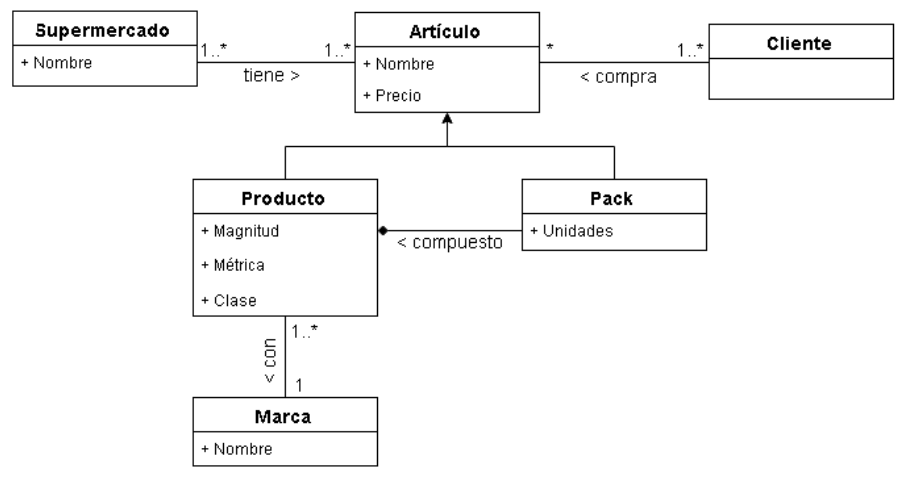
\includegraphics[height=0.30\textwidth]{dominio}
\centering
\caption{Dominio del Problema}
\end{figure}

Básicamente, un supermercado tiene un conjunto de artículos que pueden ser comprados por diversos clientes. Además, dichos artículos pueden ser de dos tipos: productos unitarios o packs de productos, asociados a una única marca que los distribuye.

La única restricción no estructural al modelo concierne a la relación “compuesto”. Según el diagrama, no sólo se trata de una agregación indicando que un pack está compuesto por una serie de productos, sino que además dichos productos pueden ser todos de diferente clase (p.e. canastas navideñas, paquetes de snacks, etc), pero es más frecuente encontrar packs de productos de una misma clase (p.e. cajas de alfajores x12, refresco Coca-Cola de 2.5L x6, etc). Los primeros, además de ser poco recurrentes son más difíciles de identificar dadas las condiciones de búsqueda (crawling), por lo que estarán fuera del alcance del proyecto, y por tal motivo serán una restricción al modelo.

Una limitación al dominio del problema refiere a las cadenas de supermercados que ofrecen servicio de compra online. En Uruguay, al corriente año 2015, sólamente dos empresas ofrecen este servicio: Devoto \cite{Devoto} y Tienda Inglesa \cite{TInglesa}. En lo que resta del proyecto, al hablar de “supermercado” nos estaremos refiriendo únicamente a estos dos.

%------------------------------------------------

\subsection{Arquitectura \& diseño de módulos}
Un segundo aspecto importante a la hora de desarrollar un sistema de información es su modularización y diseño arquitectónico, claves para obtener una solución funcionalmente correcta, clara y mantenible. Si bien se trata de dos conceptos diferentes, guardan una relación muy estrecha, ya que un buen diseño de la arquitectura se sustenta por la buena modularización del sistema.

A efectos del problema, es necesario realizar un análisis previo de las fuentes para conocer la forma en que exhiben los artículos, y por consiguiente los datos relevantes que allí subyacen, para obtener una primera aproximación a los módulos que formarán parte de nuestro sistema.

\begin{figure}[H]
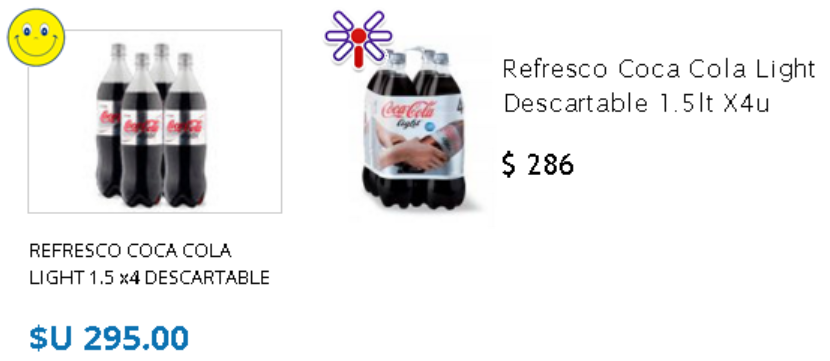
\includegraphics[height=0.30\textwidth]{coca-cola}
\centering
\caption{Formato de los Datos}
\end{figure}

En la Figura 2 se puede observar la manera en que muestran exactamente el mismo producto ambos supermercados. En ambos casos se pueden identificar tres campos; uno con una imágen ilustrativa del artículo, otro reservado para detallarlo, y otro campo dedicado a costearlo. Es fácil deducir que si bien ambos detallan el artículo de maneras muy distintas, comparten a grandes rasgos el mismo patrón. De esta forma, las etiquetas identificables en cada producto se pueden observar en la Figura 3.

\begin{figure}[H]
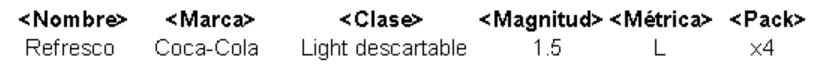
\includegraphics[height=0.07\textwidth]{etiquetas}
\centering
\caption{Etiquetas}
\end{figure}

Cabe destacar que no todas ellas son obligatorias (como el “pack”), y aunque lo sean pueden estar ausentes (como es el caso de la “métrica” en el caso de Devoto). Por otro lado, la “clase” de producto puede encontrarse dispersa en el texto de descripción. También se pueden presentar diferencias en cuanto a la sintaxis; el caso más obvio son las mayúsculas/minúsculas, pero también existen casos poco triviales como es el de “x4” versus “X4u” para indicar el pack o también “L” versus “lt” para indicar la métrica. Estos últimos dos ejemplos tienen un claro impacto en la semántica de los datos (significan lo mismo, pero están escritos de forma distinta). Un último aspecto a tener en cuenta son las magnitudes, que asociadas a determinada métrica determinan la cantidad neta de artículo, pudiendo presentar problemas de inconsistencias entre las fuentes (p.e. 0.75L o 750ml), siendo necesaria su estandarización. 

Dadas  estas condiciones, es sumamente necesario contar con un módulo que se encargue de normalizar el corpus, extraer los datos de relevancia, y etiquetarlos de acuerdo a las categorías anteriormente descritas.

Otro aspecto relevante al problema busca responder a la pregunta “¿Cómo obtener los datos del sitio web?”. Para ello, es necesario un módulo que se encargue de la extracción de datos por medio de la técnica de web-crawling, en donde se rastreen los artículos por la red que forma el sitio web mediante sus hipervínculos. Dicho módulo estará dedicado a integrar el framework de Scrapy al sistema.

Por último, debido a que el sistema a desarrollar será web, será necesario un módulo que se encargue de recibir las solicitudes de los clientes, procesarlas y retornar los resultados adecuados, renderizando dichas respuestas en formato HTML. Además, la etapa de procesamiento de solicitudes abarca dos aspectos: la normalización de los datos de entrada para ajustarse al modelo propuesto y una técnica que permita encontrar el resultado óptimo a las necesidades del cliente.

Dicho esto, y a modo de resumen, el sistema estará compuesto por cuatro módulos:
\begin{itemize}
	\item Crawler     - Encargado de la búsqueda de datos en los sitios web
	\item Parser     - Encargado de normalizar y etiquetar los datos
	\item Servidor     - Encargado de atender las solicitudes de los clientes
	\item Ranking     - Encargado de encontrar la solución óptima 
\end{itemize}


La relación entre dichos módulos incorporando la base de datos determina la arquitectura de nuestro sistema, la cual se detalla en la Figura 4.

\begin{figure}[H]
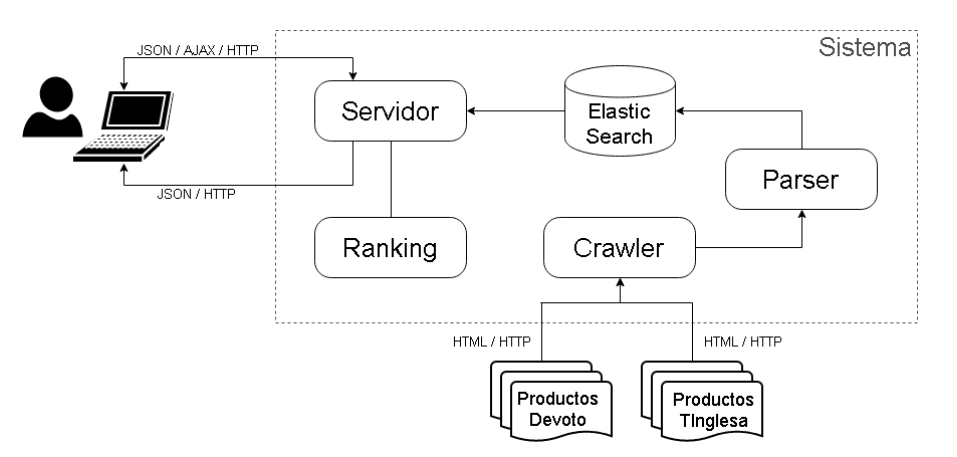
\includegraphics[height=0.30\textwidth]{arquitectura}
\centering
\caption{Arquitectura de la Solución}
\end{figure}


%------------------------------------------------

\subsection{Modelo de datos}

Un tercer aspecto importante a la hora de diseñar un sistema es describir cómo será el modelo de datos. Al contar con un buen esquema, los datos capturados y almacenados tendrán una estructura que refleja adecuadamente las entidades del mundo real y no se verán expuestos a continuas transformaciones.

En esta oportunidad se optó por modelar las entidades de la realidad descrita de la manera que se muestra en la Figura 5.

\begin{figure}[H]
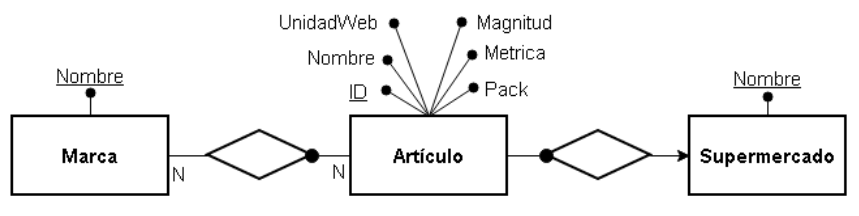
\includegraphics[height=0.20\textwidth]{modelo_de_datos}
\centering
\caption{Modelo de Datos}
\end{figure}

Son varios los detalles del modelo a destacar. El primero es que los atributos asociados al Artículo se corresponden con las etiquetas que deseamos obtener a partir de las descripciones que ofrecen los sitios web, y además un dato redundante “UnidadWeb”, que tendrá la magnitud y métrica del producto como se muestra en el sitio web. Esto último se debe al hecho de que se optó por mantener la “Magnitud” y la “Métrica” en un formato normalizado, a efectos de poder realizar los cálculos para hallar la compra óptima para el cliente de manera eficiente. Es decir, dada la heterogeneidad de representar las cantidades netas de cada artículo, se mantendrán como estándares el mili-Litro (mL) para el volumen, el Gramo (G) para la masa, o en su defecto NULL para aquellos artículos que se vendan sin estos datos. Por lo tanto, con el atributo “UnidadWeb” nos aseguramos de que el usuario pueda interactuar con las unidades de los productos en la forma que éste acostumbra. Por ejemplo, si el usuario desea un litro de leche, no sería deseable que tenga que ingresar la magnitud y métrica en el formato normalizado que utiliza el sistema (que sería 1000ml), dado que está acostumbrado a utilizar “1Lt”. Otro detalle importante es que si bien hemos mencionado que un Artículo puede ser un Producto o un Pack de productos, dichas sub-entidades se colapsaron una única entidad ya que el único atributo que lo distingue del resto es “Pack”, cuyo valor bien podría ser 1 (uno) para aquellos productos que se venden unitariamente, sin presentar mayores inconvenientes y así se ahorran costosas operaciones de “join”. Un último detalle refiere a la “clase de producto”. En esta oportunidad se optó que el atributo “Nombre” fuese conformado por el nombre del producto propiamente dicho y además la clase a la que pertenece, ya que en el sistema no hay un requisito que necesite mantenerlos diferenciados (aunque podría serlo, y ser parte de un trabajo futuro)

No obstante, este esquema estructurado aplica a un modelo relacional, y como hemos mencionado secciones anteriores se utilizará un sistema gestor de base de datos no-relacional para almacenar la información. Pese a esta disyuntiva, el esquema orientado a documentos permite, si bien no es obligatorio, mantener un esquema estructurado. Dicho esquema, no es más que un simple JSON que permite indizar los atributos y realizar consultas en forma eficiente sobre ellos. En un esquema de datos aplicado a la solución real del problema se mantiene una colección de documentos (como los mostrados en la Figura 6) por cada supermercado.

\begin{figure}[H]
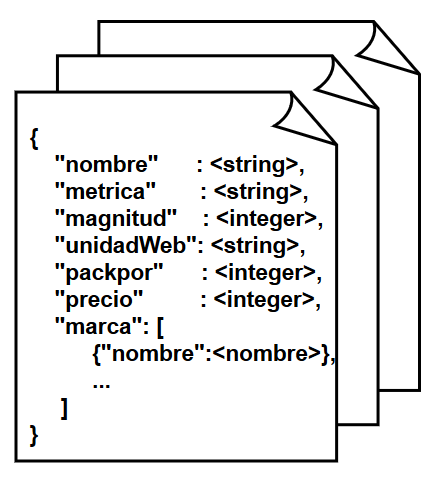
\includegraphics[height=0.30\textwidth]{documento}
\centering
\caption{Esquema de Datos DBDO}
\end{figure}

%------------------------------------------------

\subsection{Interfaz con el usuario}
Para evitar utilizar costosas técnicas de procesamiento del lenguaje natural para responder a preguntas como “¿Qué fue lo que usuario quiso decir?”, se optó por diseñar una interfaz de usuario amigable, y a la vez funcional, que contemple este amplio espectro. 

En ese sentido se optó por dejar al usuario la libertad de ingresar el nombre del producto, y restringir el resto de los atributos dependiendo de qué fue lo que ingresó el usuario.

Como puede verse en la imagen a continuación, el usuario ingresará el nombre de un producto, y para ese producto ingresado se le mostrarán las marcas que tengan alguna coincidencia en el nombre de artículo con la búsqueda ingresada. Una vez seleccionada una marca, se le desplegarán las unidades disponibles para la conjunción de los atributos. A medida que el usuario vaya ingresando las preferencias, se irán desbloqueando del mismo modo los atributos Pack, Cantidad y los checkboxes asociados (si desea que la unidad sea exacta o que el pack pueda ser desarmado).

Una vez completada toda la información para un artículo, se habilitará la opción de agregar uno nuevo, o de realizar el cálculo de cuáles son los tres productos más baratos en cada supermercado.

En la Figura 7 se muestra la página principal del prototipo con los aspectos detallados anteriormente.

\begin{figure}[H]
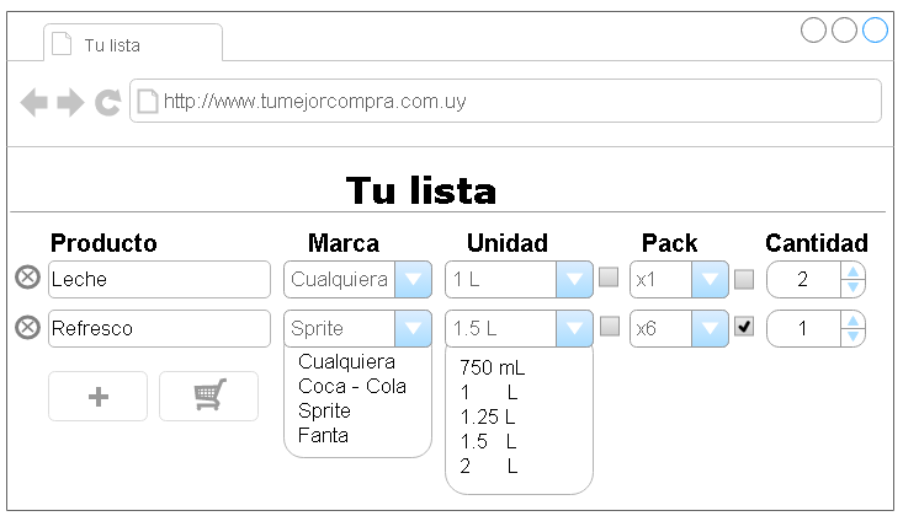
\includegraphics[height=0.30\textwidth]{interfaz_usuario}
\centering
\caption{Página Principal}
\end{figure}

Esta opción de diseño fue tomada para minimizar los posibles errores de escritura que el usuario pueda llegar a ocasionar, como por ejemplo “Hellman’s” o “Hellmans”. Una mejora a futuro sería contar con un diccionario de sinónimos y un procesamiento del lenguaje natural más fino, que permita al sistema tener la autonomía para reconocer este tipo de diferencias como el mismo artículo. Otro error que se mitiga con este tipo de control es que el usuario a priori no tiene por qué conocer la magnitud y métrica del producto que desea adquirir, pudiendo ingresar datos inexistentes, como por ejemplo un Refresco Coca Cola de 10 gr. Al habilitar las opciones una vez que se completen todos los campos, se evitan hacer costosos controles sobre todos los mismos para ver si hay algún error. Para una segunda versión, se podría dar la posibilidad de eliminar un artículo ya ingresado.

El usuario tendrá la opción de decidir si quiere que sus productos se busquen exactamente como los ingresó, o si permite que alguno de los campos se “desarmen” para encontrar otros productos que satisfagan sus necesidades y sean más económicos. 
Por ejemplo, el usuario desea comprar un pack de 6 botellas de Refresco Coca Cola de 1 litro. Si el usuario desea que su búsqueda sea exacta, el sistema le devolverá solamente los packs de 6 botellas de Refresco Coca Cola de 1 litro; si el usuario permite “desarmar” su producto, el sistema podría retornar, por ejemplo 2 packs de 3 botellas de Refresco Coca Cola de 1 litro, o 3 botellas de Refresco Coca Cola de 2 litros.


En la Figura 8, se puede ver un DSS completo sobre el caso de uso, pero a más alto nivel para describir la interacción entre el usuario y los módulos del sistema. Para una mayor usabilidad e interfaz amigable al usuario, se optó por realizar las consultas al servidor mediante AJAX de manera asincrónica. De este modo, el sitio no quedará bloqueado ni el usuario se quedará esperando por la respuesta y podrá seguir navegando sin problemas por el sitio.

\begin{figure}[H]
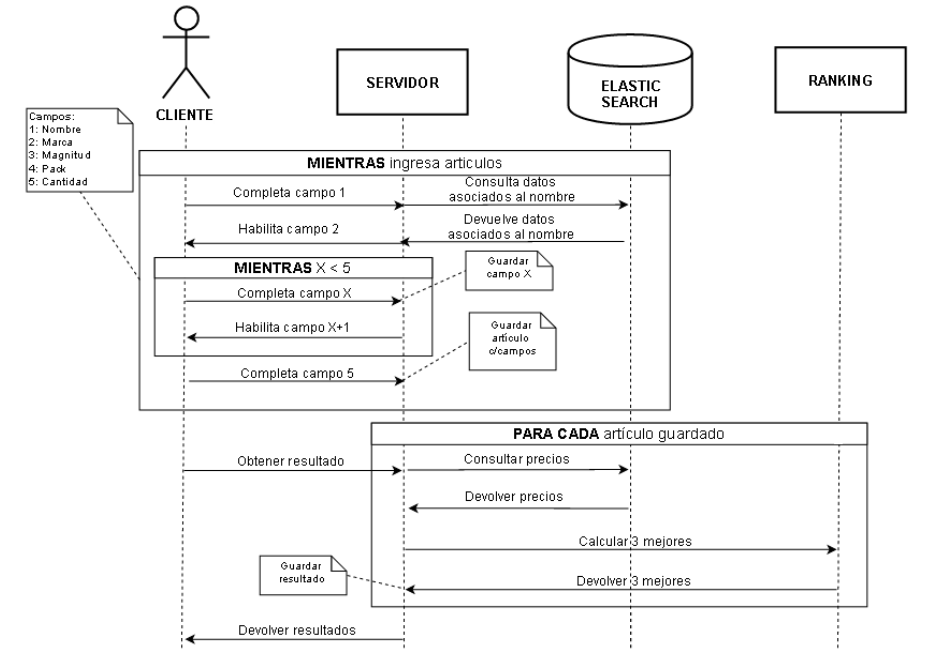
\includegraphics[height=0.40\textwidth]{DSS}
\centering
\caption{DSS}
\end{figure}

Una vez que el usuario haya finalizado con su lista de compras, podrá obtener los resultados sobre cuál supermercado es el más económico. Como puede verse en la Figura 9, para cada supermercado y para cada producto, se dan las tres posibilidades más económicas que coincidan con la búsqueda ingresada.

\begin{figure}[H]
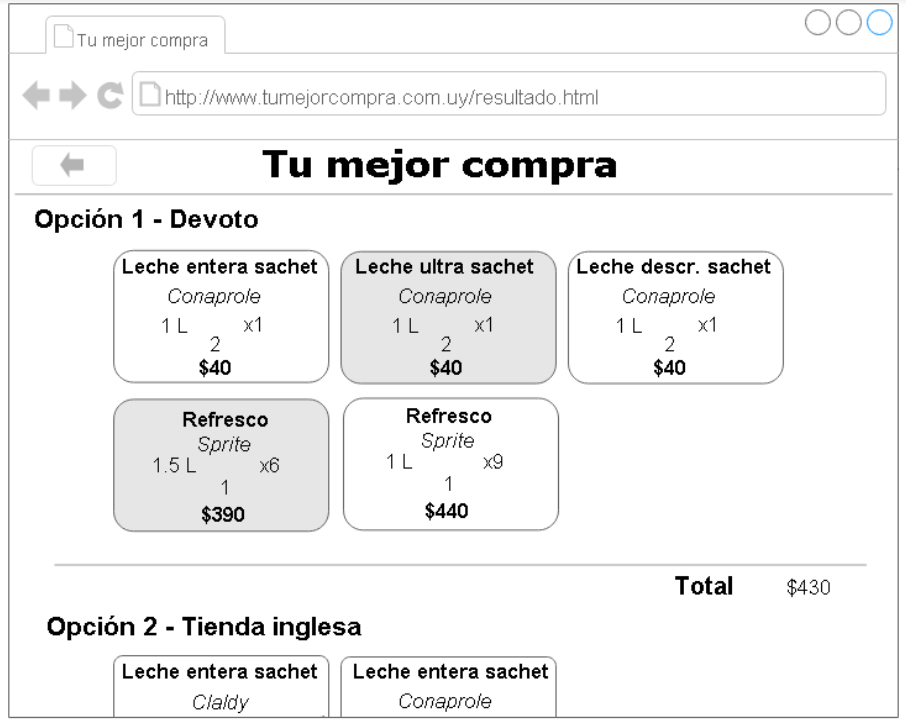
\includegraphics[height=0.30\textwidth]{pag_resultado}
\centering
\caption{Página de Resultado}
\end{figure}

Esta funcionalidad permite seleccionar entre las diferentes opciones, e ir viendo el gasto total en tiempo real. Así, en caso de que en algún supermercado no hubiera un artículo ingresado por el usuario, se dará la posibilidad de elegir uno similar. Por ejemplo, Coca-Cola 1x5lt pack x6 podría tenerlo Devoto y no Tienda Inglesa, pero que aún así el usuario prefiriera esta última opción aunque tuviera que comprarlas por separado.

%------------------------------------------------

\subsection{Recuperación de información}

%------------------------------------------------
\subsubsection{Crawler}

El crawler consiste de dos spiders, uno para cada supermercado.

El spider de Devoto \cite{Devoto} tiene como páginas base las páginas de las categorías “Vida saludable”, “Almacén”, “Frescos”, “Congelados” y “Lácteos”. Una vez en ellas, sabe como extraer los links de las subcategorías, como los que se indican en la Figura 10.

\begin{figure}[H]
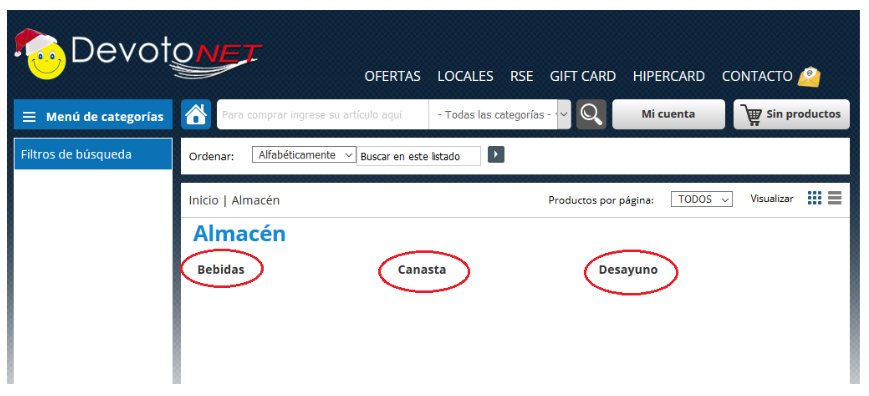
\includegraphics[height=0.30\textwidth]{pag_devoto}
\centering
\caption{Categorías Iniciales Devoto}
\end{figure}


Una vez llega a una subcategoría “hoja”, comienza a extraer los productos. Analiza los patrones en el HTML para reconocer el título y precio de un producto. Por ejemplo, a continuación se observa una versión simplificada del código HTML de un producto y en la Figura 11 su correspondiente imagen:


\begin{lstlisting}[language=HTML]
<div class="productos-categoria">
<a class="js-fancybox-product fancybox fancybox.iframe" href={URL_PROD}>
<img src={URL_IMAGEN} class="img-catproducto">
<h2>AGUA AQUARIUS MANZANA 1.5LT.</h2>
<h3>$U 50.00</h3>
<h4>U$S 1.72 </h4>
</a>
</div>
\end{lstlisting}

\begin{figure}[H]
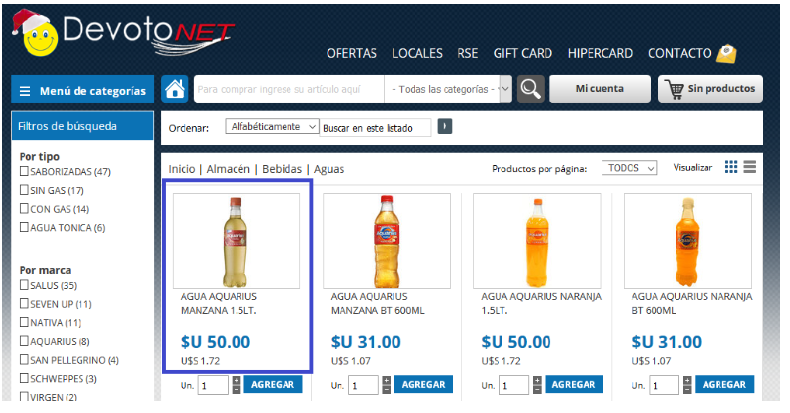
\includegraphics[height=0.30\textwidth]{producto_devoto}
\centering
\caption{Producto de Devoto}
\end{figure}


Dado que los productos están paginados, el spider debe iterar sobre todas las páginas de la categoría. Esto lo logra tomando la URL de una página, e incrementando en uno el parámetro en el cabezal HTTP que indica la página.

El spider para la página de Tienda Inglesa \cite{TInglesa} es muy similar, pero tiene una variante. Los listados de productos no tienen páginas, sino que los mismos se agrandan al scrollear hacia abajo. Dado que no se puede simular un scrolleo con Scrapy, se tuvo que encarar el problema de forma distinta. Tienda Inglesa expone un servicio web con la siguiente URL: \texttt{http://www.tinglesa.com.uy/ajax/listado/listadosPaginadoSegunScroll.php}, que es consumido por la interfaz web para agregar productos al listado a medida que se scrollea. Este servicio web retorna un HTML, que es analizado por código Javascript, que luego genera el HTML final que ve el usuario. Por lo tanto, en vez de realizar scraping sobre el HTML que ve el usuario, la solución que se implementó consume ese servicio web y parsea el HTML retornado para obtener los productos.

%------------------------------------------------
\subsubsection{Parsing}

El parsing de la información consiste de dos procesos. El primero es, dado el título de un producto en una de las páginas web, por ejemplo, ‘Alfajor Portezuelo 100 gr’, extraer la marca del mismo. Para que esto sea posible se necesita un corpus de marcas registradas. El mismo se encontró en el Catálogo de Datos Abiertos del gobierno \cite{DatosAbiertos}. A este corpus se le fueron agregando más marcas a medida que se analizaron los datos recabados de las páginas, alrededor de 287, sumando un total de 4343 marcas en el corpus. También se creó un “mini” corpus de marcas mal escritas con su correspondiente corrección, para detectar marcas mal escritas en el título de los productos.

El segundo proceso en el parsing consiste en extraer la unidad en la que se vende el producto. Por ejemplo, para el producto ‘Refresco Coca - Cola 1 Lt x6u’, el parser debe reconocer que el producto ‘Refresco Coca - Cola’ se está vendiendo con una unidad de un litro, y en packs de 6 unidades. Para lograr esto, se observaron los “patrones” que las páginas utilizan para escribir estos datos. Luego de que el parser reconoce estos patrones, se aplica un proceso de normalización, para almacenar los productos con las mismas unidades (gr o ml) y por ende facilitar la posterior comparación.

%------------------------------------------------
\subsubsection{Base de Datos}
La estructura de la base de datos queda definida de la siguiente forma servidor/indice/tipo. En nuestro caso tenemos un índice por cada supermercado y un único tipo que son los productos. 
Básicamente se realizan dos tipos de operaciones: almacenamiento de datos y consulta de datos. 
\\
\\
\textbf{Almacenamiento de datos}
\\
ElasticSearch carga los datos a partir de un servidor, un índice, un tipo y un dato. 
A partir del parseo de datos, se obtiene un archivo que contiene un conjunto de JSONs (como los mencionados en la sección Modelo de Datos) y para cada elemento se realiza un request de tipo POST a la base de datos para almacenarlo.
\\
\\
\textbf{Consulta de datos}
\\
Dado que ElasticSearch está pensado como un servidor de búsqueda, tiene gran flexibilidad para realizar consultas y búsquedas. Analicemos el caso en que el usuario estuviera buscando un producto con las siguientes propiedades:
\begin{itemize}
	\item nombre: Alfajor de chocolate
	\item marca: Portezuelo
	\item unidad: 100gr
	\item packpor: x12
\end{itemize}

El sistema generaría la siguiente consulta en formato JSON:
$
	{\\
       query: {\\
          bool: {\\
             must: [\\
                { match: { nombre: { query: “Alfajor de chocolate”, operator: “and” } } },\\
                { match_phrase: { marca: “Portezuelo” } },\\
                { match: { unidad: “100gr” } },\\
                { match: { packpor: 12 } }\\
             ]\\
          }\\
       }\\
   }\\
$


El campo bool indica las condiciones que debe cumplir el objeto para satisfacer la consulta. Puede contener elementos de tipo \textit{must}, \textit{must\_not} y \textit{should}. Dado que sólo estamos usando un subcampo must, todo objeto que cumpla las condiciones dentro de él será válido.

Dentro del \textit{must} se observan cuatro condiciones. La primera indica que se está buscando un producto cuyo nombre contenga las palabras “alfajor”, “de” y “chocolate”. Esto es gracias al operador \textit{and}. Si esto no fuera así, se podrían perder resultados valiosos para el usuario. Si hubiera un producto en la base llamado “Alfajor de sabor chocolate” y no se estuviera usando el operador \textit{and}, la consulta no devolvería ese producto ya que el servidor buscaría los productos cuyo nombre contenga el substring completo. El segundo campo expresa la marca que se está buscando, y el \textit{match\_phrase} indica que la marca debe ser exactamente la buscada. Si existiera una marca llamada “Portezuelo 2”, los productos con ella no serían devueltos. Los últimos dos campos indican la unidad y el pack buscados, respectivamente.

%------------------------------------------------

\subsection{Estrategia de ranking}
El último requisito para cumplir con la especificación del sistema es definir el mecanismo que realizará el ranking de artículos que satisfagan las necesidades indicadas por el cliente. 

Para cumplir con dicho objetivo, se optó por deducir una relación numérica entre los componentes que determinan un determinado artículo. Más precisamente, la relación antes dicha debe vincular por un lado la magnitud, las unidades por pack y la Cantidad requerida por el cliente, y por otro la magnitud y unidades por pack provistas por los supermercados, todas ellas en función de la exactitud de la magnitud o la posibilidad de desarmar un pack (a opción del cliente). 

En otras palabras, la intención es buscar la cantidad real de determinado artículo en función de los parámetros antes dichos, resultando de esta forma la siguiente ecuación:

\[
cantidad(Q,M,P) =
\begin{cases} 
\frac{Q\times M\times P}{M_T \times P_T} & exacto \wedge \neg desarmable \wedge Q\times M\times P\ mod\ M_T \times P_T = 0 \\ 
\frac{Q\times P}{P_T} &  \neg exacto \wedge \neg desarmable \wedge Q\times P\ mod\ P_T = 0 \\
\frac{Q\times M}{M_T} & exacto \wedge desarmable \wedge Q\times M\ mod\ M_T = 0 \\
Q & \neg exacto \wedge desarmable \\
\infty & en otro caso


\end{cases}
\] 

donde los parámetros $Q$, $M$ y $P$ definen la cantidad, magnitud y unidades por pack indicados por el usuario respectivamente, mientras $M_T$ y $P_T$ representan la magnitud y unidades por pack disponible en la tienda para ese artículo.

Finalmente, una vez hallada la cantidad real necesaria para satisfacer las necesidades del cliente, se multiplican por el precio impuesto por la cadena de supermercados y se ordenan en forma creciente. Dicha solución se restringe a los primeros tres artículos, de forma de satisfacer los requisitos detallados en la sección referente a la interfaz de usuario.

%----------------------------------------------------------------------------------------
%	PROBLEMAS ENCONTRADOS Y TRABAJO FUTURO
%----------------------------------------------------------------------------------------

\section{Problemas encontrados y trabajo futuro}

%------------------------------------------------

\subsection{Crawler}

En la actualidad muchas páginas cargan contenido de forma dinámica mediante AJAX. Este fue uno de los principales problemas que tuvimos que resolver a la hora de obtener los datos de la web. Para resolver este problema fue necesario hacer que el spider de Scrapy haga requests directamente a los servicios Web que devuelven el contenido. En el anexo se agrega el código con indicaciones de dónde se encuentra este problema.

%------------------------------------------------

\subsection{Mejorar corpus de marcas}
Los supermercados pueden incorporar nuevos productos, con marcas que no están en el corpus, o pueden ya existir productos cuyas marcas no están en el mismo o están mal escritas y por ende la aplicación no las reconoce. Es un claro camino de mejora el de agrandar el corpus de marcas, así como agrandar el corpus de marcas mal escritas.

%------------------------------------------------

\subsection{Mayor procesamiento para detectar sinónimos y palabras mal escritas.}
Gran parte del valor de la aplicación es la capacidad de comparar los precios de dos productos equivalentes. Para lograr esto, el sistema debe poder reconocer cuando dos productos son iguales. Se observó que esta tarea es de gran dificultad dadas las diferencias en la manera de escribir los títulos de los productos. Algunas de estas diferencias pueden ser: el uso de sinónimos (bebida y refresco, por ejemplo), faltas de ortografía, caracteres inesperados y palabras vacías. Puede significar una gran mejoría para la aplicación la habilidad de reconocer estas diferencias y normalizarlas, para distinguir con más precisión cuando se está tratando del mismo producto. Esto se podría lograr con alguna herramienta de procesamiento de lenguaje natural, como Freeling.


%----------------------------------------------------------------------------------------
%	CONCLUSIONES
%----------------------------------------------------------------------------------------

\section{Conclusión}

En este proyecto nos enfrentamos a algunas de las dificultades más importantes que tiene la recuperación de la información en la web, los errores humanos. Por más distante que sea la interacción de quién crea la página web con la interfaz que llega al usuario final, de una forma u otra es una persona la que termina ingresando datos, o eligiendo el formato en que se muestran. Esto lleva a que los datos no siempre sean correctos ni del todo homogéneas, y por lo tanto se dificulte el procesamiento automático de los mismos.

Otro aspecto importante a destacar, es la relación entre áreas necesaria para poder realizar un proyecto de estas características. Sin lugar a dudas, el proyecto tiene una carga importante de Procesamiento del Lenguaje Natural, y orientado a esta área es que se encuentran la mayor parte de las mejoras propuestas.

\section{Anexo}


\newpage
%----------------------------------------------------------------------------------------
%	BIBLIOGRAFÍA
%----------------------------------------------------------------------------------------

\begin{thebibliography}{1}
\bibitem{Scrapy} \textit{http://scrapy.org/, último acceso, Noviembre 2015}
\bibitem{Scrapy2} \textit{http://www.inqbation.com/es/extraiga-informacion-de-cualquier-web-facilmente-con-scrapy/, último acceso, Noviembre 2015}
\bibitem{ElasticSearch} \textit{https://www.elastic.co/products/elasticsearch, último acceso, Noviembre 2015}
\bibitem {Devoto} \textit{http://devoto.com.uy/, último acceso, Diciembre 2015}
\bibitem {TInglesa} \textit{http://tinglesa.com.uy/, último acceso, Diciembre 2015}
\bibitem {DatosAbiertos} \textit{https://catalogodatos.gub.uy/dataset/habilitacion-registro-alimentos/resource/9a7ebeca-7990-4db4-aea2-5477a3c14e2b, último acceso, Octubre 2015}

\end{thebibliography}

%----------------------------------------------------------------------------------------

\end{document}